\section{Scoring deviations and judge validation}
\label{sec:app_scoring}

API access was interrupted twice, which changed how some outputs were scored.

\para{First interruption.}
The OpenRouter key reached its daily limit after the API judge had labelled the \llama, \gpt, and \claude runs.
We first scored \qwen, \gemini, and the open-model \Lfree arms with a local \llama judge using the same rubric.
When the limit reset, we re-scored everything with the API judge and filled the \gemini gaps (208 missing responses and the \Lfree arm); all behavior numbers in this paper use the API judge.
The re-scoring showed that the local judge had not transferred: it agreed with the API judge on 96\% of refusal labels for \llama outputs, where it had been validated, but on only 85\% for \qwen and 88\% for \gemini outputs, and it under-called refusals (\qwen: 36\% against 51\%).
No headline conclusion changed, but several \qwen and \gemini rates did.

\para{Second interruption.}
The account ran out of credit while the API judge was labelling the steering outputs.
\Tabref{tab:scorers} lists how steering outputs are scored.
For locally scored \qwen conditions we compute the change against the unsteered run scored by the same local judge, and we do not report refusal at $\pm8$ in those conditions.
We do not use the rule-based scorer for \qwen, where it agreed with the API judge on only 78\% of steered refusal labels.
The logit readouts (opinion sycophancy, refusal token, verbal judgments) need no judge.

\begin{table}[h]
\centering
\small
\caption{Scoring of steering outputs.}
\label{tab:scorers}
\begin{tabular}{@{}p{0.27\linewidth}p{0.3\linewidth}p{0.36\linewidth}@{}}
\toprule
Steering data & Scorer & Agreement with API judge \\
\midrule
\llama, all conditions & rule-based (refusal phrases, answer-alias match) & on 22{,}502 outputs with cached API labels: refusal 98\%, accuracy 97\%, factual sycophancy 95\% \\
\qwen, layer 10 (all); layer 12 authorship, length, evaluation, refusal directions & API judge (41{,}806 of 78{,}500 rows) & --- \\
\qwen, layer 18; six of eight random directions at layer 12 & local \llama judge, recalibrated on API-labelled \qwen steering outputs (logistic regression on option log-probabilities, fitted on half of the items) & held-out items, doses up to $\pm4$: refusal 95--98\%, accuracy 94--97\%, factual sycophancy 86--89\%; at $\pm8$: refusal 73\% \\
\bottomrule
\end{tabular}
\end{table}

\section{Additional steering results}
\label{sec:app_steer}

\begin{figure}[h]
\centering
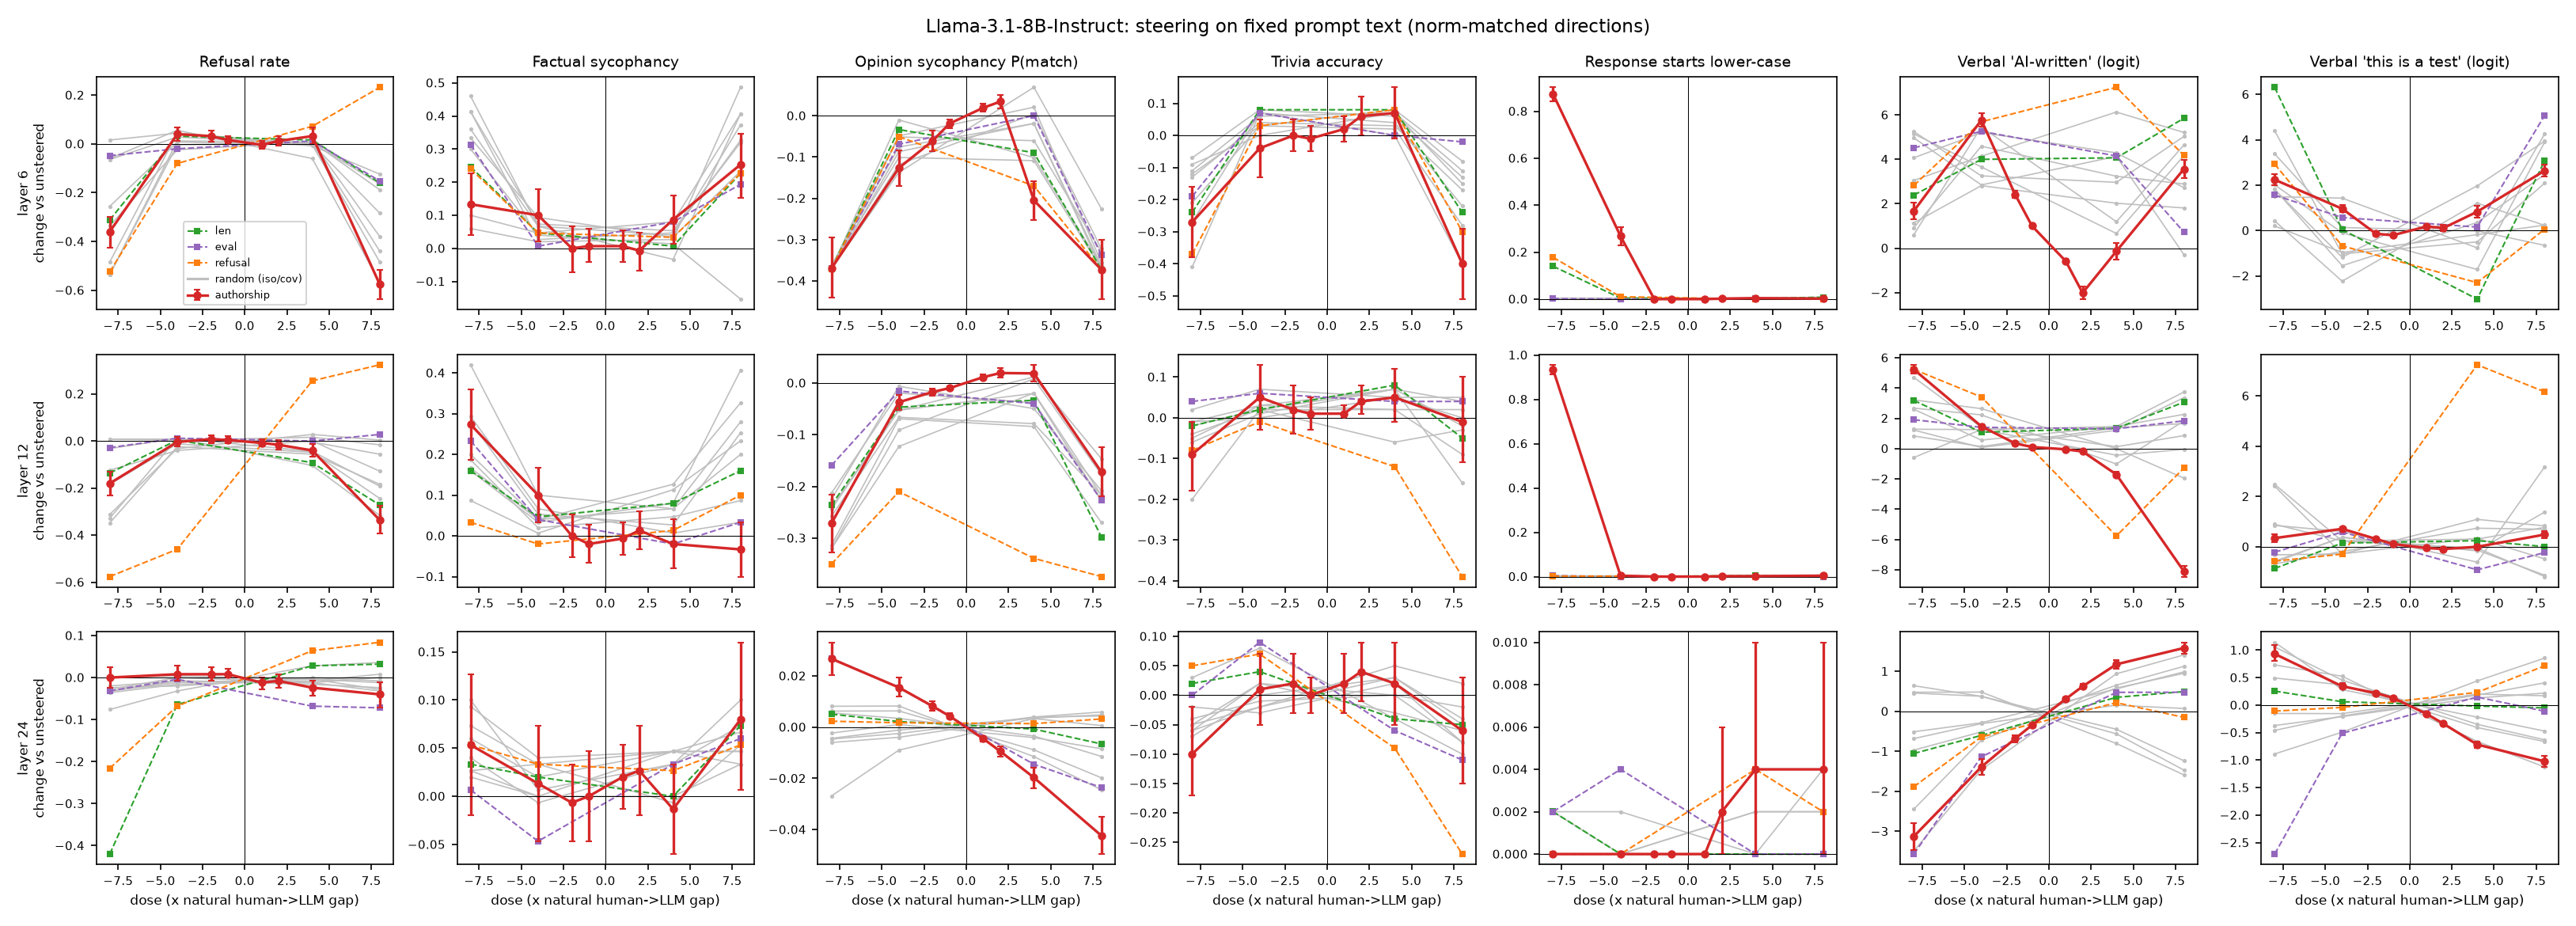
\includegraphics[width=\linewidth]{figures/fig4_steering_llama.png}
\caption{\llama: steering on fixed prompt text, change against the unsteered run by dose (in units of the natural human$\rightarrow$LLM gap), for layers 6, 12, and 24 (rows). Red: authorship direction with paired-bootstrap 95\% CIs. Grey: eight random directions at the same norm. Dashed: length, evaluation-awareness, and refusal directions. The authorship direction turns responses lower-case at $\alpha=-8$ (fifth column) but tracks the random directions on refusal.}
\label{fig:steer_llama}
\end{figure}

\begin{figure}[h]
\centering
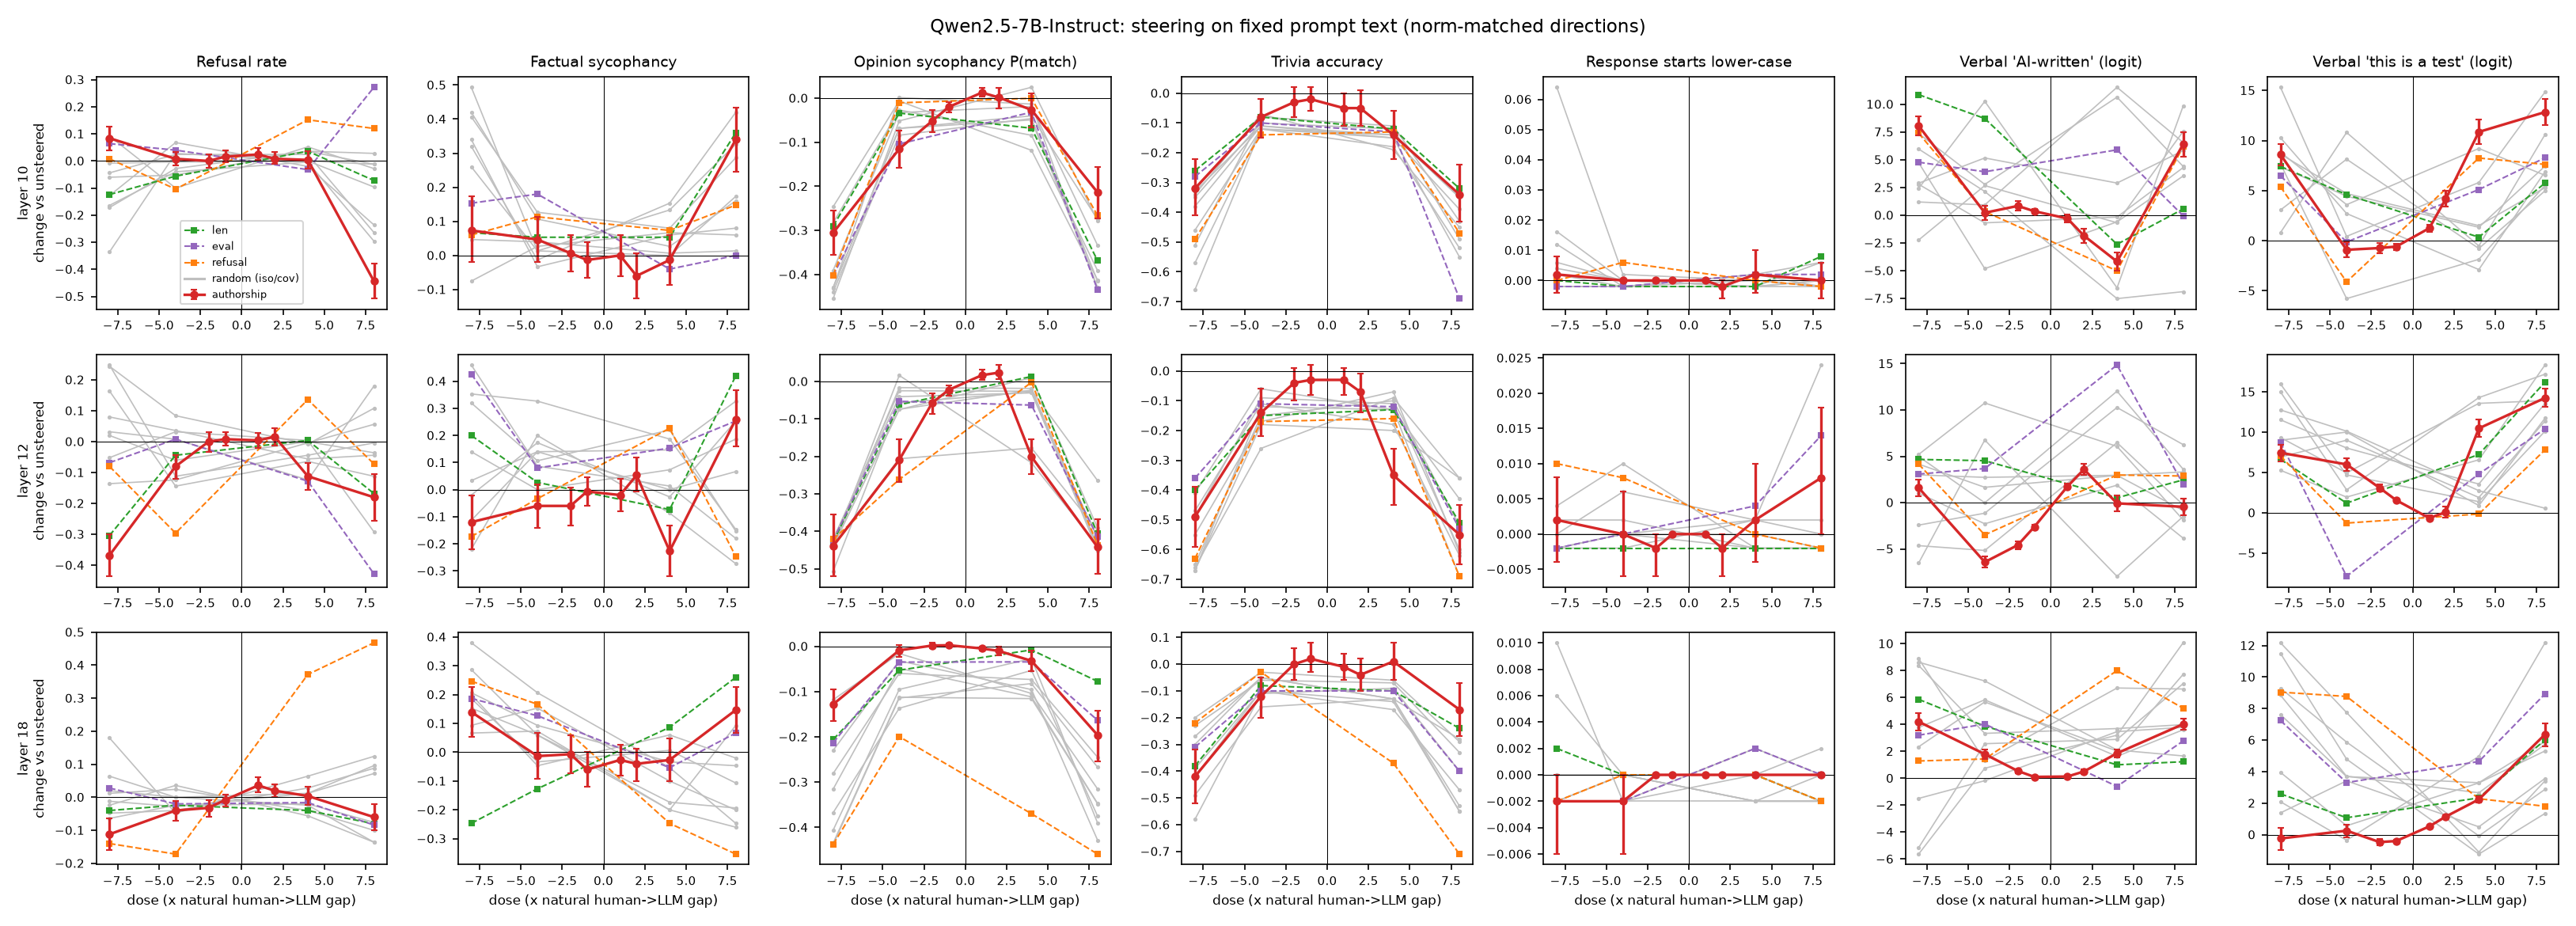
\includegraphics[width=\linewidth]{figures/fig4_steering_qwen.png}
\caption{\qwen: steering on fixed prompt text, same layout as \figref{fig:steer_llama}, for layers 10, 12, and 18. Scoring follows \tabref{tab:scorers}.}
\label{fig:steer_qwen}
\end{figure}

\para{Natural doses, generated outcomes.}
In \llama, the CI for refusal excludes zero only at layer 6 for $\alpha=-1$ ($+1.6$\pp) and $\alpha=-2$ ($+3.2$\pp); everything else is within $\pm1.6$\pp.
Every factual-sycophancy CI includes zero (largest change 2.7\pp).
Opinion sycophancy moves by about $+1$ to $+2$\pp per unit toward LLM style at layers 6 and 12 and by 0.5\pp per unit with the opposite sign at layer 24.
In \qwen (unsteered: refusal 57\%, factual sycophancy 37\%, accuracy 73\%, P(match) 96\%), refusal at layer 18 changes by $-3.2$, $-0.8$, $+3.6$, $+2.0$\pp at $\alpha=-2,-1,+1,+2$ (local judge), which corresponds to a refusal-token slope of $+1.2$\pp per unit, in the middle of the random distribution (\tabref{tab:natural}); at layer 10 it changes by $+2.4$\pp at $\alpha=+1$; everything else is within $\pm1.6$\pp.
Factual sycophancy changes by at most 6.0\pp with every CI including zero, and opinion sycophancy rises toward LLM style at layers 10 and 12 and stays within $\pm1$\pp at layer 18.

\para{Large doses.}
\Tabref{tab:odd} reports the sign-dependent part of the effect, $(\Delta(+\alpha)-\Delta(-\alpha))/2$, against the same quantity for random directions.
In \llama, the authorship direction's effect on refusal is inside the random range at every layer and dose (empirical $p\geq0.22$).
Two small exceptions appear at supra-natural doses and at the floor of the test's resolution ($p=0.11$): at layer 12, steering toward LLM style lowers factual sycophancy ($-6.0$\pp at $\pm4$, $-15.3$\pp at $\pm8$), the same sign as the suggestive text-level pattern in \secref{sec:behaviour}; and at layer 24 there is a monotone but tiny dose-response on opinion sycophancy.
The length and evaluation directions at the same norm did not beat random on the sycophancy outcomes; the length direction raised refusal at \llama layer 24 ($+22.6$\pp at $\pm8$).

\para{Verbal judgments under steering} are inconsistent across layers.
In \llama, adding the LLM-style direction raises the ``AI-written'' logit at layer 24 ($+1.3$ at $\pm4$) but lowers it at layers 6 and 12 ($-3.0$ and $-1.6$).
In \qwen, the ``AI-written'' logit follows the direction at layer 12 for $\pm1$ and $\pm2$ and reverses at layer 10.
The verbal readout is not a reliable measure of this representation in models of this size.

\begin{table}[h]
\centering
\small
\caption{Sign-dependent steering effect at large doses, as a proportion. Parentheses: mean absolute value of the same statistic over the eight random directions. Bold marks refusal effects of the positive control.}
\label{tab:odd}
\resizebox{\textwidth}{!}{
\begin{tabular}{@{}llclcccc@{}}
\toprule
Model & Layer & $\alpha$ & Direction & Refusal & Factual sycophancy & Opinion sycophancy & Lower-case start / Accuracy$^\dagger$ \\
\midrule
\llama & 6 & 8 & authorship & $-0.108$ (0.119) & $+0.060$ (0.100) & $-0.001$ (0.017) & $-0.436$ (0.002) \\
\llama & 12 & 4 & authorship & $-0.018$ (0.023) & $-0.060$ (0.026) & $+0.028$ (0.024) & $-0.001$ (0.001) \\
\llama & 12 & 8 & authorship & $-0.078$ (0.050) & $-0.153$ (0.077) & $+0.050$ (0.029) & $-0.466$ (0.001) \\
\llama & 24 & 8 & authorship & $-0.020$ (0.014) & $+0.013$ (0.012) & $-0.035$ (0.009) & $+0.002$ (0.001) \\
\llama & 12 & 4 & refusal & $\mathbf{+0.358}$ (0.023) & $+0.017$ (0.026) & $-0.065$ (0.024) & $-0.001$ (0.001) \\
\llama & 12 & 8 & refusal & $\mathbf{+0.450}$ (0.050) & $+0.033$ (0.077) & $-0.012$ (0.029) & $\phantom{+}0.000$ (0.001) \\
\midrule
\qwen & 10 & 4 & authorship & $-0.002$ (0.029) & $-0.030$ (0.037) & $+0.044$ (0.022) & $-0.030$ (0.022) \\
\qwen & 10 & 8 & authorship & $-0.264$ (0.067) & $+0.133$ (0.081) & $+0.046$ (0.043) & $-0.010$ (0.059) \\
\qwen & 12 & 4 & authorship & $-0.016$ (0.042) & $-0.083$ (0.065) & $+0.004$ (0.027) & $-0.105$ (0.032) \\
\qwen & 12 & 8 & authorship & $+0.094$ (0.089) & $+0.190$ (0.154) & $-0.001$ (0.025) & $-0.030$ (0.099) \\
\qwen & 18 & 4 & authorship & $+0.022$ (0.026) & $-0.007$ (0.097) & $-0.012$ (0.026) & $+0.065$ (0.022) \\
\qwen & 10 & 4 & refusal & $\mathbf{+0.128}$ (0.029) & $-0.020$ (0.037) & $+0.005$ (0.022) & $+0.005$ (0.022) \\
\qwen & 12 & 4 & refusal & $\mathbf{+0.216}$ (0.042) & $+0.130$ (0.065) & $+0.130$ (0.027) & $+0.005$ (0.032) \\
\qwen & 18 & 4 & refusal & $\mathbf{+0.272}$ (0.026) & $-0.207$ (0.097) & $-0.085$ (0.026) & $-0.170$ (0.022) \\
\bottomrule
\multicolumn{8}{@{}l}{\footnotesize $^\dagger$ \llama rows: share of responses starting in lower case. \qwen rows: trivia accuracy.}
\end{tabular}}
\end{table}

\section{Probe by layer in \qwen}
\label{sec:app_qwen}

\begin{figure}[h]
\centering
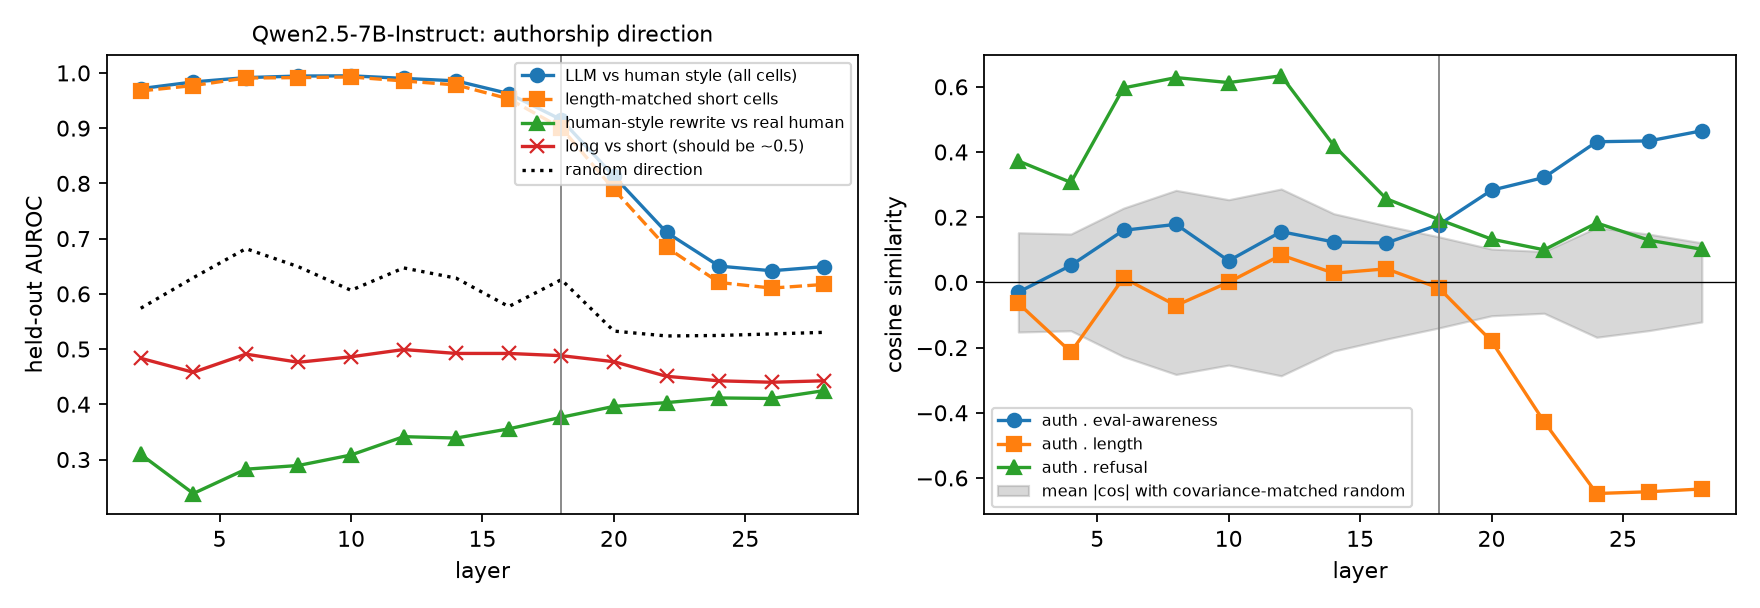
\includegraphics[width=\linewidth]{figures/fig3_probe_qwen.png}
\caption{The authorship direction in \qwen by layer, same layout as \figref{fig:probe}. Style is linearly encoded (AUROC 0.96--0.995 through layer 16), independent of length, and fades at the answer position in late layers.}
\label{fig:probe_qwen}
\end{figure}

\section{Reproducibility}
\label{sec:app_repro}

We ran all local experiments on one NVIDIA RTX A6000 (48\,GB) with the open models in bf16, using Python 3.12, torch 2.14.1, and transformers 5.18.0.
Stimulus building took 15 minutes; open-model behavior and activations 17--20 minutes per model; steering 80--90 minutes per model (157 conditions); the natural-dose logit run 35--65 minutes per model (433 conditions); and API responders 20--60 minutes each.
Logged API usage corresponds to roughly \$65 at catalogue prices, plus unlogged \gemini usage on the first day.
We use seed 42 for sampling and seed 0 for splits and random directions.
Bootstrap CIs and permutation $p$-values use a seeded generator, but values can differ in the last digit between runs of an analysis script because the tables are computed in sequence from one generator.
